\chapter{\label{cha:c11tester}Fuzzing with C11Tester}

C11Tester is a automatic testing tool that supports a large gragment of C/C++ weak memory model. This chapter presents an overview of C11Tester and customazation points of its plugable framework. Then the fuzzer's implementation is described. Finally we show the evaluation results on some of the benchmarks.

\section{Overview of C11Tester}

The C11Tester contains the following basic constructs: insstrumentation, scheduler, consistency checker and race detecter.

C11Tester uses a LLVM pass compiler pass, CDSPass, to instrument all atomic operations, non-atomic accesses to shared memory locations, thread functions, mutex operations and fence operations by inserting a corresponding function call. The compiled program is linked with a dynamic library containing the function calls.
C11Tester impelments a thread library that supports the same APIs of C++'s standard library and Posix thread library. The user's thread function calls will be mapped into user space fibers, instead of kernel space threads. Thus, all threads will be executed in a sequential manner with scheduling managed by a central scheduler, which is provided by the C11Tester. A context switching approach is applied to simulate the interleavings of threads to improve efficiency.
Each atomic operation, thread creation and joining, mutex locks and unlocks, and memory fences will create a Action object, containing its type, value, memory order, thread id and other runtime information. Since all threads are sequenced during execution, each action will have a unique sequence number. The relations between actions, such as read from and synchronized with, are also maintained by the Action class.

Although C/C++ programs under weak memory model do not use scheduling semantics, C11Tester does contain a central scheduler. It's worth noting that the scheduler do not simulate schedulings of threads, instead, it's designed to check actions of different threads in a total order. This is based on the implementation of mapping user's threads into fibers and checking them sequentially. All actions within the same thread will be checked following their sequence order, as a step, and the scheduler decides whether to check actions of other threads in the next step. Hence, two decisions will be made in each step, the behavior of the current action and the next thread to select. If the current action is a read, C11Tester will choose a write action to read from. Since the read-modify-write operations are instrumented with two functions, a read and a write, the scheduler ensures these two actions are atomic, i.e. to check them without switching to other threads in between.

Memory locations are devided into two types: atomic locations and non-atomic locatios. Non-atomic access to shared memory locations is the source of introducing data races. C11Tester implements a race detecter to check data races. The race detecter will allocate a chunk of shadow memory for each of the non-atomic memory locations. Loading from or writing to non-atomic shared variables are instrumented with specific functions, which will register the current thread's state to the shadow memory. When multiple concurrent access to some shared non-atomic memory with at least one of them being a write is detected, a data race will be reported.

Here we use an example to demonstrate the process of C11Tester's model checking procedure.

\begin{lstlisting}[caption={P3}, label={P3}]
#include "librace.h"
#include <atomic>
#include <thread>
uint8_t data = {};
std::atomic<int> flag = { 1 };  

// thread 2
void t2() {
    store_8(&data, 0);          // cds_store8    
    flag.store(1, mo_release); 
}

// thread 3
void t3() {
    if (flag.load(mo_acquire))
        store_8(&data, 1);
}

// thread 1
int main() {
    std::thread thrd2(t2);
    std::thread thrd3(t3);
    thrd2.join();
    thrd3.join();
}
\end{lstlisting}

In this program, there are two shared variables: non-atomic variable data and atomic flag. The librace.h header is provided by C11Tester, containing the instrumented function store\_8 for non-atomic variables. The initialization of flag, which is non-atomic, deliberately uses 1 as the initial value. Since the c++ standard thread library internally calls POSIX APIs, the thread-related function calls will be hooked by C11Tester's dynamic library.

After compilation, the model checker launches the program. After initializing the global variables, the model checker creates the first thread, which is the main thread and assign an tid, 1, to it. The first event is creating thrd2. After thrd2 is created and assigned an tid of 2, two threads, main and thrd2, are active. The model checker will randomly pick a thread to continue. Suppose the main thread is selected, the next event of it is creating thrd3. After creating thrd3, the next event of main is joining thrd2, so it becomes inactive. Now the current active threads are: thrd2 and thrd3.

If the model checker selects thrd2, the two events in it, writing to data and flag, will be consumed, and the thrd2 is finished. Now thrd2 becomes joinable and the currently active threads are: main and thrd3. Suppose main is selected and after joining thrd2 it becomes inactive again. Then thrd3 becomes the only active thread so it will be executed without the need to make a choice. The first event in thrd3 is loading the value of flag. Since the store of flag in thrd2 has already been explored, the non-atomic initialization of flag is hidden in the modification order. Hence only the atomic store is visible to this load, and the rf relation also forms a synchronization-with relation between the two thread. When writing to the non-atomic data, the race detecter checks pervious access to that location. The store in thrd2 happens before the read in the current thread, which happens before the current store, so all events are totally ordered and no data race will be reported.

Considering another case, suppose the model checker selects thrd3 after creating both threads. The load of flag will be executed and only the initialization of data is visible to it. After reading the initial value, the store of data is consumed. When thrd3 is finished, the stores in thrd2 will be executed. When writing to data, the race detecter checks previous actions relating to that memory location. The store in thrd3 is already explored and it has no happen before relations with the current store, so the two stores are concurrent and a data race is reported.

One optimization that C11Tester implements is that it will consume writes with release and relaxed memory orders, only pausing on sc writes. This is because the sc order is part of the C/C++11 memory model so different sc order will result in different executions. Besides, consuming the weak writes will not lose the ability to cover possible executions. Consider the following example  \ref{P4},
\begin{lstlisting}[caption={P4}, label={P4}]
    std::atomic<int> var = {};      // (w0)
    void t2() {
        auto _ = var.load(acquire); // (r1)
    }
    void t3() {
        var.store(1, sc);           // (w1)
        var.store(2, release);      // (w2)
        var.store(3, release);      // (w3)
    }
\end{lstlisting}
after creating two threads, if t2 is selected first, r1 can only read from the initial value. If t3 is selected, the first event, w1, in this thread will be executed. The next two events are release writes, so the model checker will not re-select threads after w1. Instead, it will execute w2 and w3 until t3 is finished. Then it finds the only active thread is t2, so it selects t2. Now the set of available writes for r1 to read from becomes: w1, w2 and w3, and r1 is free to randomly select one of them. Although making thread decisions after each event is also feasible, the optimized version is more efficient and still able to cover all 4 possible executions.

Another optimization performed by C11Tester is that it avoids backtracking during exploration. To achieve this, it performs consistency checking at each step to ensure it's valid. It make decisions based on the implications of the memory model and already explored events. In \ref{P4} for example, if t3 has been explored, when choosing the rf relation for r1 in t2, the rf-set only contains w1, w2 and w3, where w0 is excluded. If r1 had selected w0 and the model checker continues until some point where the execution graph is found to be infeasible under the memory model, it would have to perform backtracking to make a different choise for r1. Consider another example \ref{P5},
\begin{lstlisting}[caption={P5}, label={P5}]
    std::atomic<int> var = {};      // (w0)
    void t2() {
        auto _1 = var.load(acquire); // (r1)
        auto _2 = var.load(acquire); // (r2)
    }
    void t3() {
        var.store(1, sc);           // (w1)
        var.store(2, release);      // (w2)
        var.store(3, release);      // (w3)
    }
\end{lstlisting}
if r1 has already seelcted w3 to read from, only w3 will be included in the rf-set for r2, becuase w3 $\xrightarrow{\text{rf}}$ r2 implies that w0-2 are modification-ordered before w3 and thus should not be visible to r2, which is sequence ordered after r1. Otherwise the RR coherence will be violated. Excluding infeasible writes from the rf-set ensures the rf's to be valid, which in turn avoids the backtracking efforts.

To summarize, C11Tester will execute the program from beginning to end, randomly picking threads and writes, with the optimizations of consuming weak writes and constraining rf-sets.


\section{Customazation points of C11Tester}

C11Tester provides two interfaces: selectWrite and selectThread that randomly selects a thread or write from a provided set. These two functions can be overwritten to implement new fuzzers. The provided set already excludes invalid choices so it's safe to pick other choices in the set. Thus we can define two types of mutations: changing the next thread to be added or changing the write that a read event reads from.

\section{Fuzzer implementation}

To implement a fuzzer described in Algorithm \ref{fuzzer}, there are several specific functions to be defined:

\begin{itemize}
	\item A hash function that computes a unique identifier for an execution graph, which is used to indicate whether the execution graph has been encountered before and to count the number of unique executions that are found in the end of N iterations.
	\item A function that returns a boolen that indicates whether the execution graph is interesting.
	\item A function that mutate the previous execution graph and produces a prefix of the mutated graph.
	\item A function that enforces the prefix, i.e. replays until the mutated choice.
\end{itemize}

The hash function for executioin graph encodes: event types, memory orders, reads-from relations. It first iterate threads by their thread ids, and for each event in each thread, it computes the hash of its event type and memory order (for atomic operations). If the event is a read event, it also combines the hash of the write event it reads from. To be noticed, in this hash function the modification order is not included although it's part of the execution graph under many memory models. This is because the hash function only cares about observable behaviours, such as read values, which may be influenced by modification orders. However, changing some modification orders may or may not change the observable behaviours. The hash function is defined in Algorithm \ref{c11fuzzer-hash} as follows:


\begin{algorithm}
	\caption{Hash of execution graphs}
	\label{c11fuzzer-hash}
	\begin{algorithmic}
		\STATE \textbf{Input:} Execution graph $g$
		\STATE \textbf{Output:} Hash value $h$

		\STATE h $\leftarrow$ 0
		\FOR{each $i$ from 0 to g.max\_tid()}
		\STATE events = g.get\_events\_in\_thread(i)
		\FOR{each $e$ $\in$ events}
		\STATE h $\leftarrow$ hash\_combine(h, e.type)
		\STATE h $\leftarrow$ hash\_combine(h, e.memory\_order)
		\IF{e is a read event}
		\STATE h $\leftarrow$ hash\_combine(h, e.rf)
		\ENDIF
		\ENDFOR
		\ENDFOR
		\RETURN $h$
	\end{algorithmic}
\end{algorithm}

The is\_interesting function returns true if the hash of the current execution graph is not covered in previous explorations. This is the least restrictful metric, alternatively, it can be defined as returning true if new rf relations has been covered. Another possible definition is to check whether the execution graph reveals a new bug, which is biased on searching for bugs. In our definition, we aims to find more new executions, with more new buggy executions being a by-product.

The mutate function uniformly picks a fixed number of decisions, including threads and rf's, with multiple choices in the provided set. For each of them, it mutates the selected decision and cuts out the rest decisions to produce a prefix. Since the only two places where randomness is used are selectWrite and selectThread, the choices of threads and writes will be uniquely mapped to an execution graph. Hence the prefix of a decision trace also defines a prefix of an execution graph.

% 画图

The mutated prefixes will be added to a prefix set. The replaying function choose a prefix from the set and enforce C11Tester to make the same decisions in that prefix. After enforcing the prefix,  C11Tester is switched to the random mode, continuing random exploration until the graph is completed.

\section{Benchmarks}

The fuzzer and C11Tester are tested under 11 benchmarks: barrier, chase-lev-deque, mpmc-queue, linuxrwlocks, mcs-lock, dekker, rwlock, seqlock, bipartite-buf, left-right and ring-buf. Some of them are collected from open source libraries, others come from the original C11Tester's benchmark set, which are also taken from open source libraries, internet discussions and papers. Here is a list of descriptions of these benchmarks:

\paragraph{barrier} It comes from a solution of StackOverflow discussion. It implements a spinning barrier that halts a fixed number of threads to wait and releases the barrier when all threads are waiting. It maintains a counter for the number of threads that are waiting so far and a step state that counts the number of barrier synchronizations. It was injected with a bug of using the relaxed memory order of the counter.

\paragraph{chase-lev-deque} An implementation of the Chase-Lev deque data structure using the C11 primitives. It was published in \cite{chase-lev-deque-impl} but found to have bug in its implementation, due to the use of relaxed operations of fences.

% TODO: ref
\paragraph{mpmc-queue} A multi-producer multi-consumer queue implementation from a blog post \cite{mpmc-queue-impl}.

\paragraph{linuxrwlocks} A reader-writer lock implementation from the Linux kernel. An rwlock only allows one writer at a time but can allow multiple readers to access the protected data.


\paragraph{mcs-lock} A list-based contention-free lock originally proposed by Mellor-Crummey and Scott\cite{mcs-lock}. The implementation comes from \cite{mcs-lock-impl}. In this data structure, each thread maintains a node of a queue. When a thread wants to lock, it asks the mutex to set its tail of the queue to be the thread's node. When other threads lock, they have to wait for the tail to be removed by the mutex.

\paragraph{dekker} A Dekker's critical section algorithm implemented with fences \cite{dekker-fence-impl}. This algorithm ensures only one thread can enter critical section at a time. A shared turn variable records which thread is taking the turn. Each thread has a flag variable to indicate its state. Before entering the critical section, a thread should first raise its own flag and then check whether the turn is not set. All atomic operations on the turn and flags are relaxed but fences are used to synchronize concurrent accesses.

\paragraph{rwlock} Another rwlock implementation similar to linuxrwlocks.
\paragraph{seqlock} A sequence lock implementation. The lock protects some shared data using an atomic counter, initialized 0. A writer increments the counter twice, both in the beginning and end of writing. Hence whenever the counter is odd, there must be some other thread modifying the data, so other threads have to wait.

\paragraph{bipartite-buf} A single-producer-single-consumer test for a bipartite buffer implementation written in C++11, customazed from \cite{lockfree-DNedic}. The bipartite buffer is a variation of the ring buffer which allows in-place processing with linear space guarantee.

\paragraph{left-right} A generic implementation \cite{lockfree-xenium} of the LiftRight algorithm\cite{left-right}. The algorithm functions similarly to the reader-writer lock, but ensures non-blocking for reads. It uses two instances for the protected data, one of which is used for all reader threads. The writer thread will work on the other instance and after writing is finished, two instances are switched.


\paragraph{ring-buf} A ring buffer that supports adding or removing multiple objects simultaneously \cite{lockfree-DNedic}. It maintains two indexes, a read and a write index of the buffer. After adding or removing, these two indexes will be updated to appropriate values.


\burcu{TODO: Briefly describe each benchmark}

\section{Evaluation and discussion}

\burcu{TODO: List the research questions you explore, and answer the questions using your experimental results.}
\burcu{Do you have some results for the larger benchmarks in C11Tester?}



\paragraph*{Research questions} The following research questions are list for evaluating the fuzzing algorithm.
\begin{enumerate}[label=RQ\arabic*]
	\item Is the fuzzer able to cover a larger range of execution graphs comparing to other random-based exploration strategies? \label{RQ:coverage}
	\item When the program has bugs, will being able to detect more bugs come as a byproduct of covering more execution graphs \label{RQ:bug}
	\item How does the fuzzer cause overhead in C11Tester in real-world applications? \label{RQ:overhead}
\end{enumerate}

To address the research questions, we use the benchmarks to test our fuzzer and other approaches with same amout of iterations, $N$, and compare their results. If not specifically stated, $N = 10000$.

\subsection{\ref*{RQ:coverage}: Fuzzer vs C11Tester}

Using the 11 benchmarks, we evaluate the ability of finding unique execution graphs of both the fuzzer and C11Tester. The metric used is the number of different execution graphs discovered over $N$ iterations. Table \ref{c11fuzzer-bench1} and \ref{c11fuzzer-bench2} show the number of unique executions found by two approaches. It can be seen that the fuzzer is able to find a larger number of different execution graphs in a fixed number of iterations than C11Tester with the random-based searching strategy in most of the benchmarks, with the average improvement of 27.0\%. The improvements are calculated by:
\[
    R_{improvement} = \frac{N_{c11Fuzzer} - N_{c11Tester} }{N_{c11Tester} } \times 100 \% ,
\]
where $N_{c11Fuzzer}$ and $N_{c11Tester}$ are the number of unique execution graphs found by C11Tester and C11Fuzzer, respectively. 

\begin{table}[h!]
	\begin{tabular}{ |c|ccccc| }
		\hline
		Benchmarks  & barrier & chase-lev-deque & mpmc-queue & linuxrwlocks & mcs-lock \\
		\hline 
		C11Tester   & 6969    & 6244            & 4185       & 981          & 9703     \\
		C11Fuzzer   & 7741    & 8505            & 6373       & 1225         & 9994     \\
		\hline
        Improvement & 11.1\%  & 36.2\%          & 52.3\%     & 24.9\%       & 3.0\%     \\
        \hline
	\end{tabular}
	\caption{benchmarks (1)}
	\label{c11fuzzer-bench1}

\end{table}

\begin{table}[h!]
	\begin{tabular}{ |c|cccccc| }
		\hline
		Benchmarks  & dekker & rwlock-test & seqlock-test & bipartite-buf & left-right & ring-buf \\
		\hline 
		C11Tester   & 395    & 9998        & 6137         & 297           & 5378       & 328      \\
		C11Fuzzer   & 494    & 9997        & 7962         & 340           & 6678       & 576      \\
		\hline
        Improvement &25.1\%  & -0.0\%     & 29.7\%        & 14.5\%        & 24.2\%     &75.6\%\\
        \hline
	\end{tabular}
	\caption{benchmarks (2)}
	\label{c11fuzzer-bench2}
\end{table}


In addition, Figure \ref{cover-plot1-barrier} to \ref{cover-plot1-ring-buf} draws the coverage plots for each benchmark, with orange lines representing the fuzzer and blue lines representing the random tester. It can be obeserved that in all of these cases the fuzzer is able to find more unique executions. In addition, in some benchmarks, see Figure \ref{cover-plot1-chase-lev-deque} or \ref{cover-plot1-mpmc-queue} for example, the fuzzer's speed of finding executions (the slop of coverage plost) is not significantly slowing down as the number of found executions grows. Some coverage plots of the fuzzer, such as in Figure \ref{cover-plot1-bipartite-buf} and \ref{cover-plot1-ring-buf}, also have some "bumps" which the random tester do not have. Such bumps are caused by some prefixes that guides to a group of new interesting executions.

\begin{figure}[H]

	\centering
	\begin{minipage}{0.45\textwidth}
		\centering
		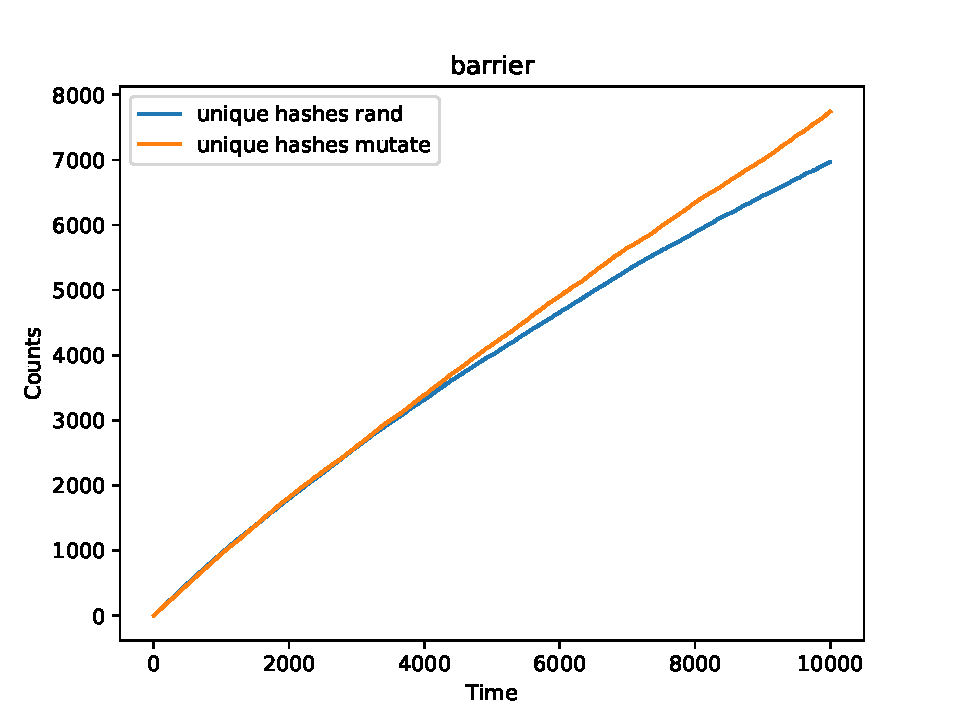
\includegraphics[width=\textwidth]{figure/barrier.pdf}
		\caption{barrier}
		\label{cover-plot1-barrier}
	\end{minipage}
	\hfill
	\begin{minipage}{0.45\textwidth}
		\centering
		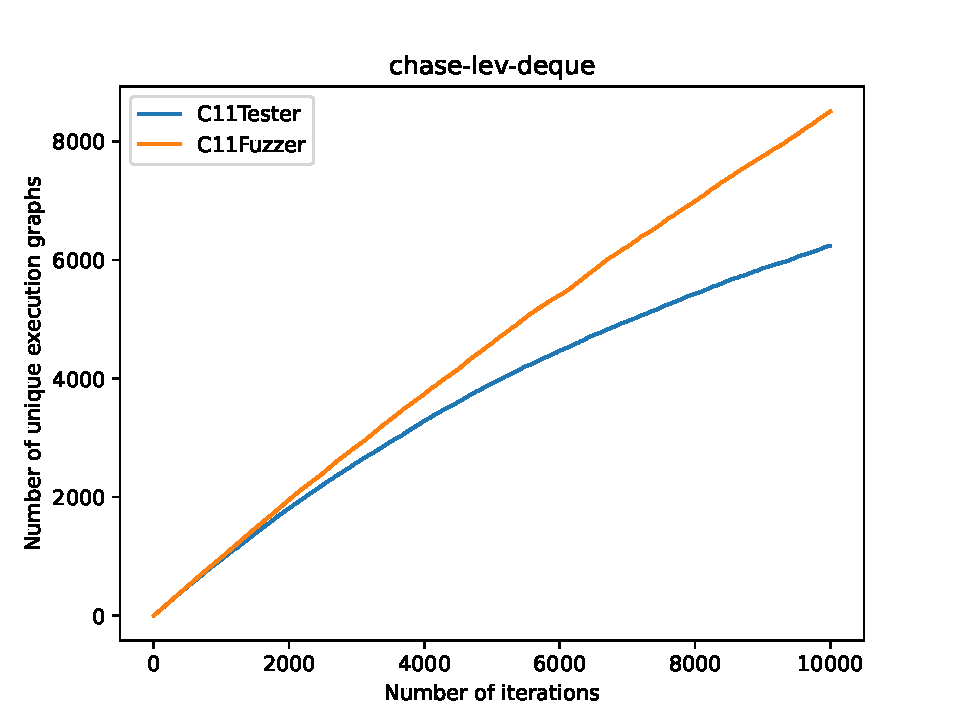
\includegraphics[width=\textwidth]{figure/chase-lev-deque.pdf}
		\caption{chase-lev-deque}
		\label{cover-plot1-chase-lev-deque}
	\end{minipage}

	\vspace{0.5cm}

	\begin{minipage}{0.45\textwidth}
		\centering
		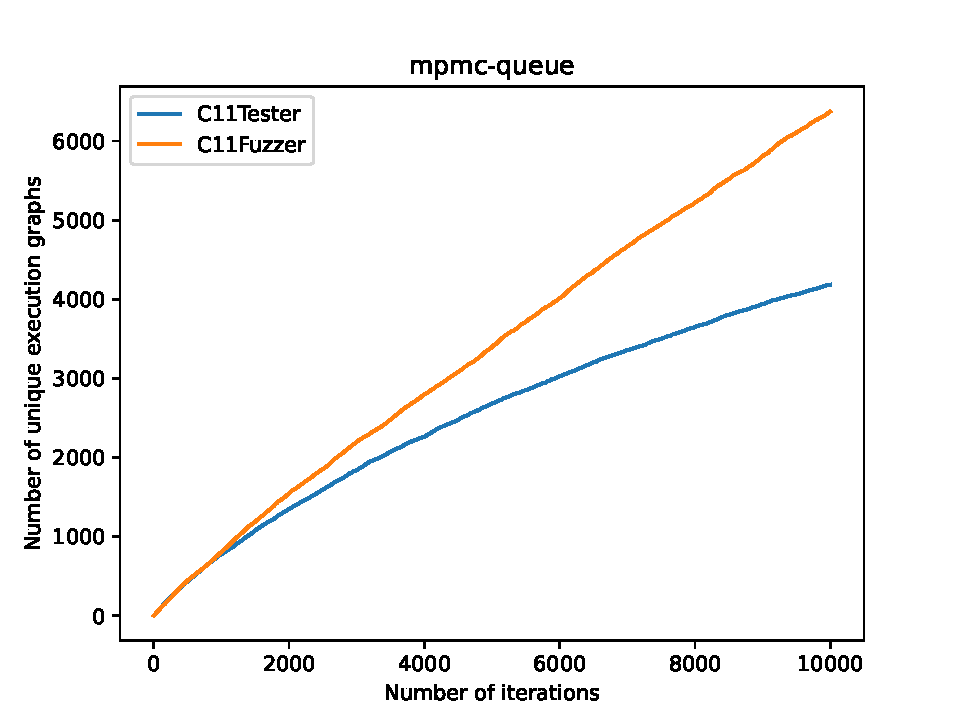
\includegraphics[width=\textwidth]{figure/mpmc-queue.pdf}
		\caption{mpmc-queue}
		\label{cover-plot1-mpmc-queue}
	\end{minipage}
	\hfill
	\begin{minipage}{0.45\textwidth}
		\centering
		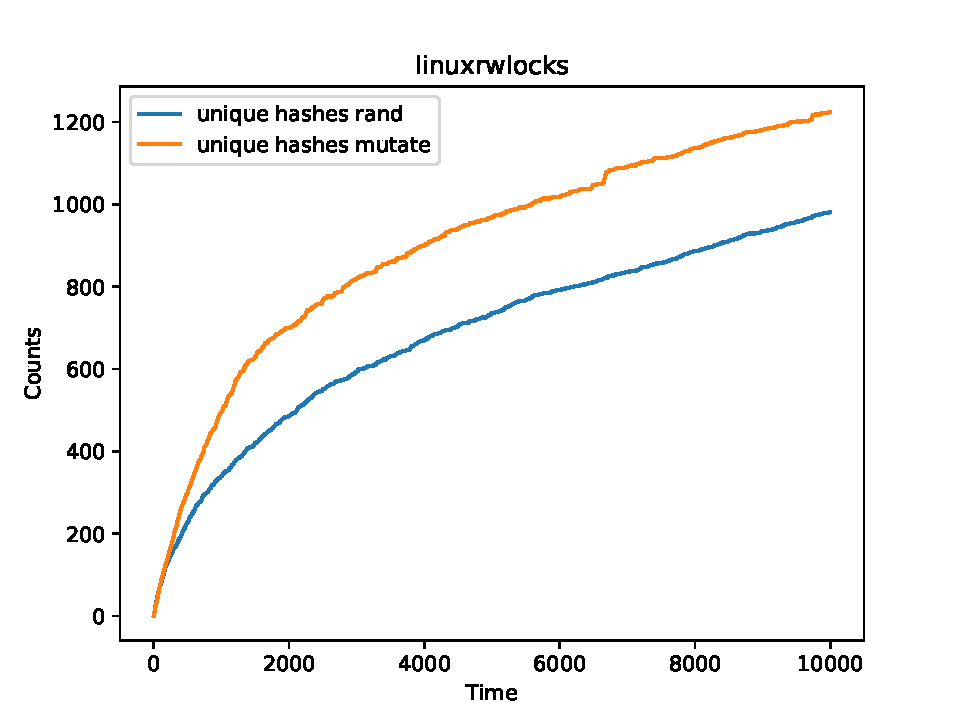
\includegraphics[width=\textwidth]{figure/linuxrwlocks.pdf}
		\caption{linuxrwlocks}
		\label{cover-plot1-linuxrwlocks}
	\end{minipage}

	\vspace{0.5cm}

	\begin{minipage}{0.45\textwidth}
		\centering
		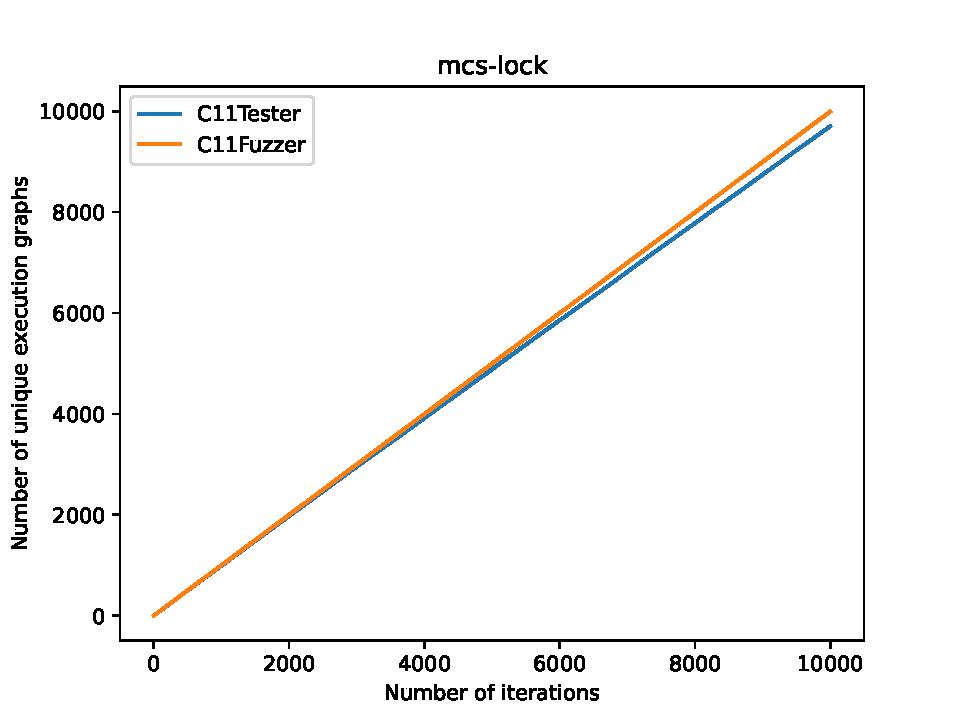
\includegraphics[width=\textwidth]{figure/mcs-lock.pdf}
		\caption{mcs-lock}
		\label{cover-plot1-mcs-lock}
	\end{minipage}
	\hfill
	\begin{minipage}{0.45\textwidth}
		\centering
		% This empty minipage will help the last image to be aligned to the left
	\end{minipage}



\end{figure}



\begin{figure}[H]
	\centering
	\begin{minipage}{0.45\textwidth}
		\centering
		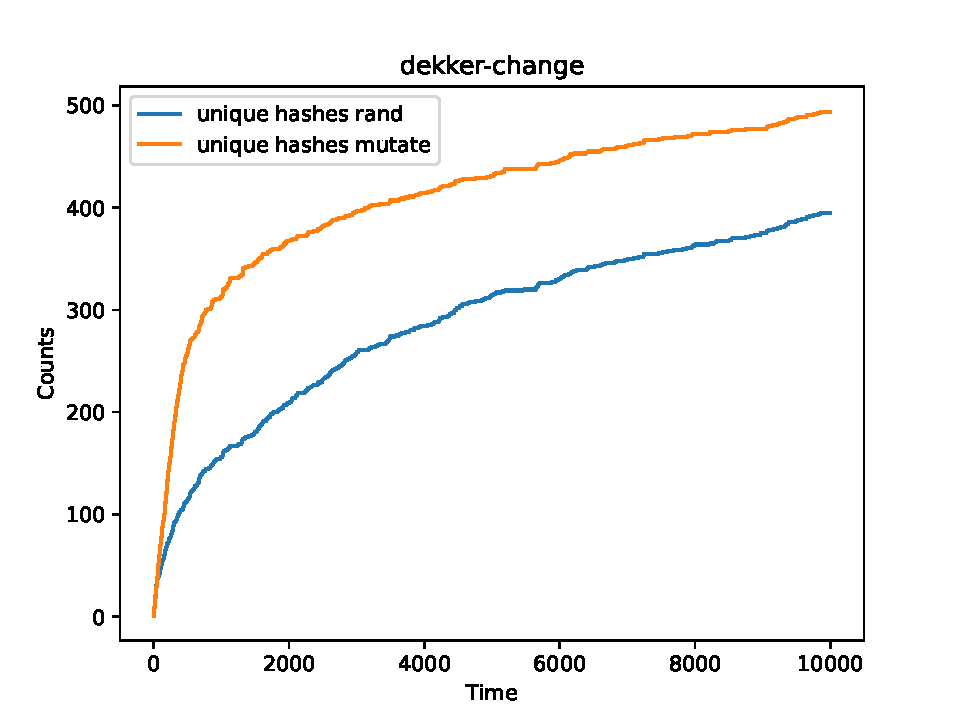
\includegraphics[width=\textwidth]{figure/dekker-change.pdf}
		\caption{dekker-change}
		\label{cover-plot1-dekker-change}
	\end{minipage}
	\hfill
	\begin{minipage}{0.45\textwidth}
		\centering
		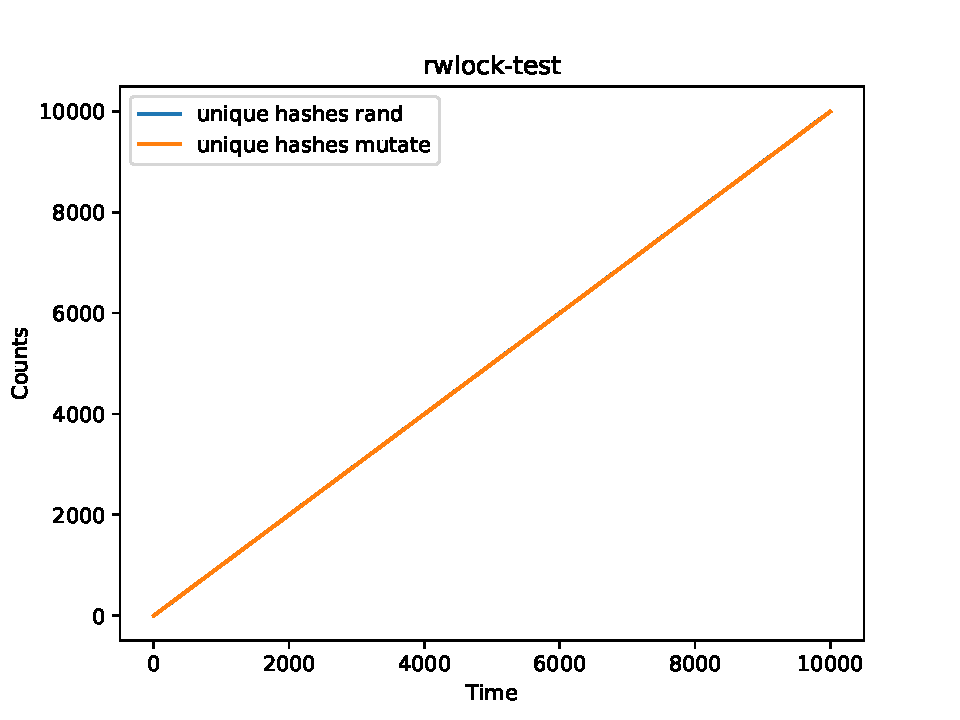
\includegraphics[width=\textwidth]{figure/rwlock-test.pdf}
		\caption{rwlock-test}
		\label{cover-plot1-rwlock-test}
	\end{minipage}

	\vspace{0.5cm}

	\begin{minipage}{0.45\textwidth}
		\centering
		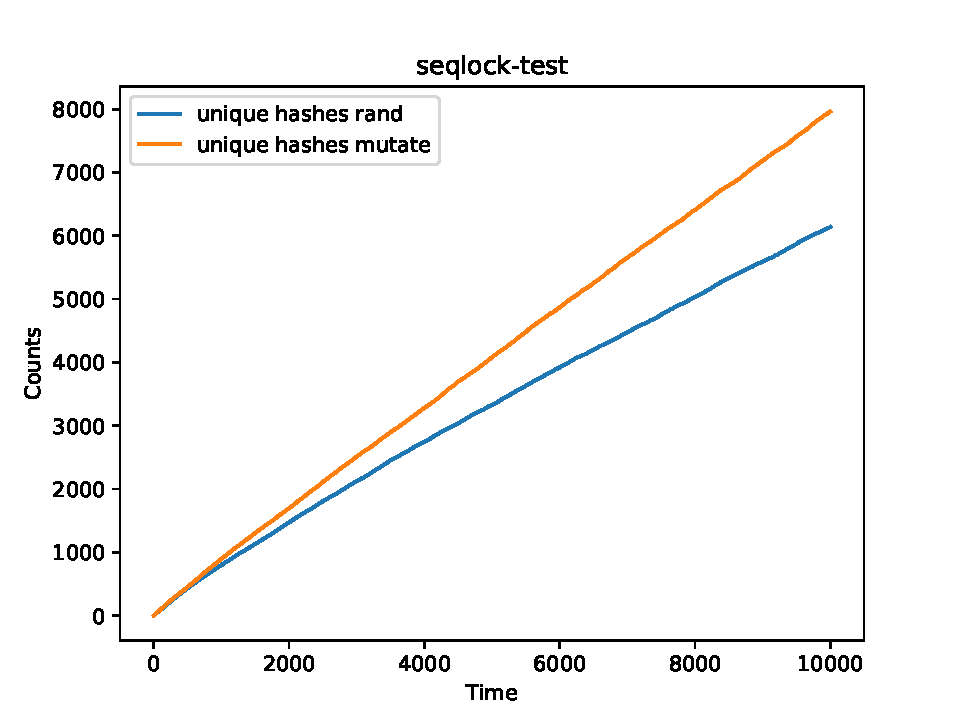
\includegraphics[width=\textwidth]{figure/seqlock-test.pdf}
		\caption{seqlock-test}
		\label{cover-plot1-seqlock-test}
	\end{minipage}
	\hfill
	\begin{minipage}{0.45\textwidth}
		\centering
		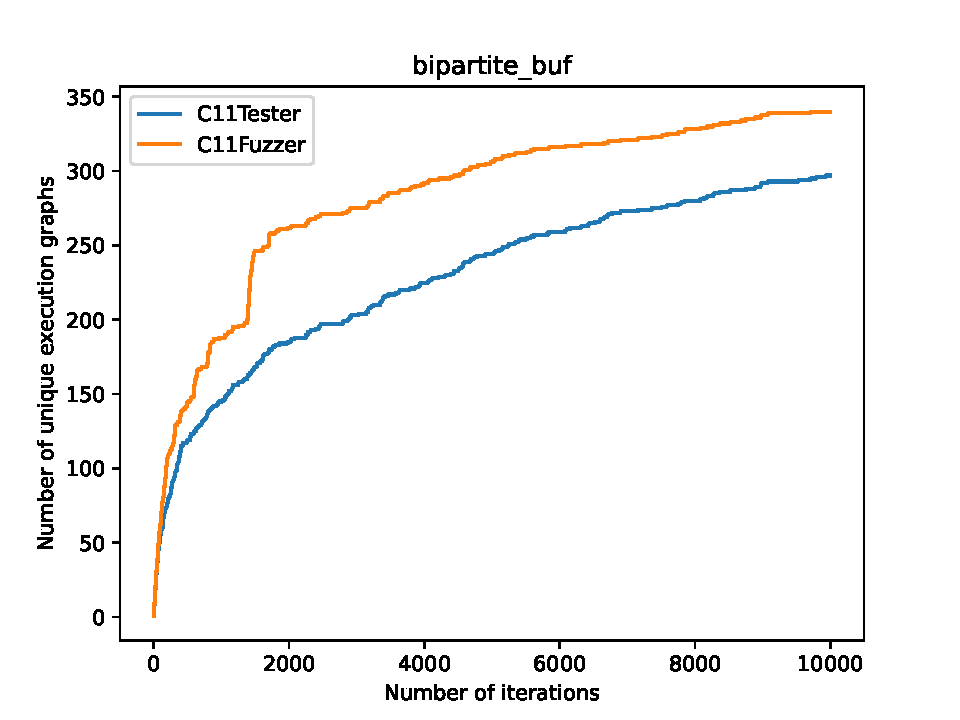
\includegraphics[width=\textwidth]{figure/bipartite_buf.pdf}
		\caption{bipartite-buf}
		\label{cover-plot1-bipartite-buf}
	\end{minipage}

	\vspace{0.5cm}

	\begin{minipage}{0.45\textwidth}
		\centering
		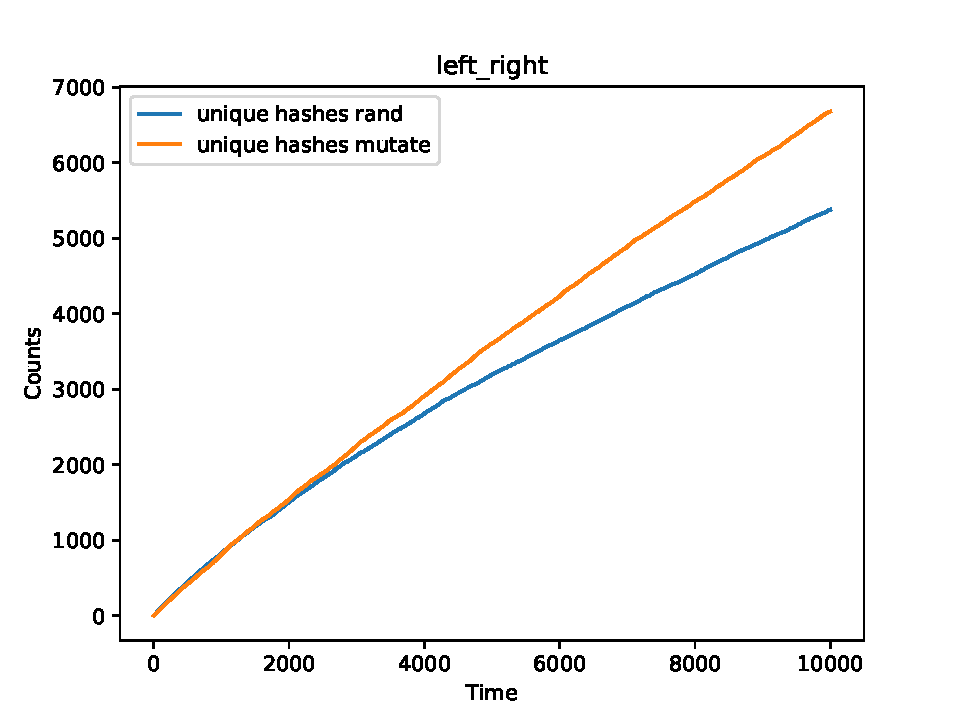
\includegraphics[width=\textwidth]{figure/left_right.pdf}
		\caption{left-right}
		\label{cover-plot1-left-right}
	\end{minipage}
	\hfill
	\begin{minipage}{0.45\textwidth}
		\centering
		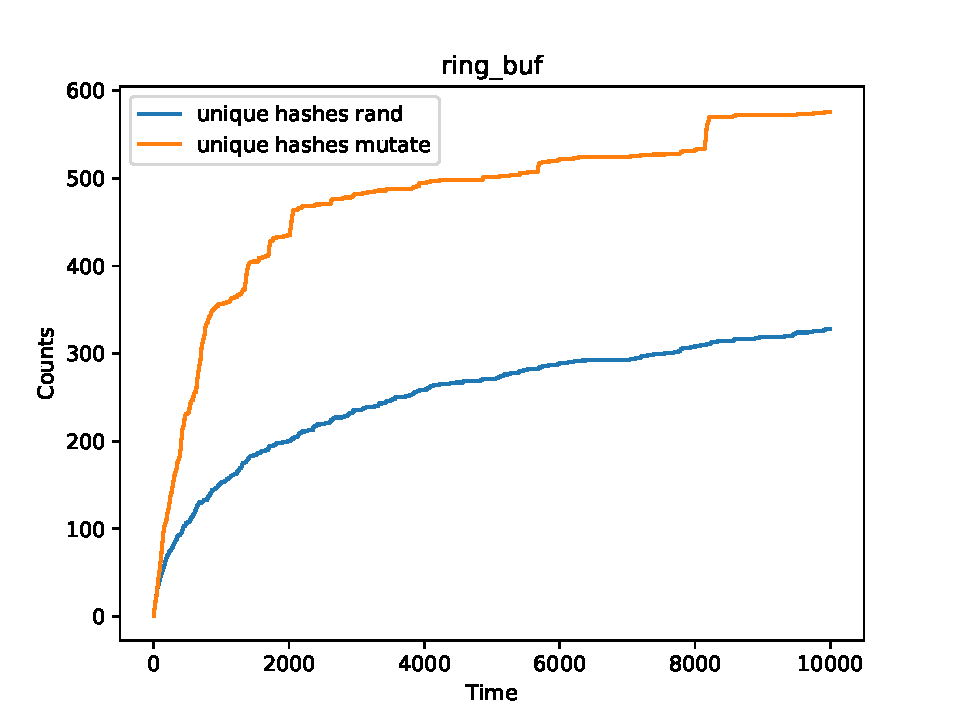
\includegraphics[width=\textwidth]{figure/ring_buf.pdf}
		\caption{ring-buf}
		\label{cover-plot1-ring-buf}
	\end{minipage}

\end{figure}

\subsection{\ref*{RQ:coverage}: C11Fuzzer vs PCTWM}

PCTWM \cite{pctwm} is a state-of-art weak concurrency tester that expands the idea of PCT, which constrains the cope of exploring executions. It is expected that PCTWM should cover a smaller range of execution graphs than that of C11Tester, which performs an unbounded random search. A subset of the benchmarks described above a tested with the same configurations of bug depth and communication events, shown in Table \ref{pctwm-configs}. 

\begin{table}[h]
	\begin{tabular}{ |c|ccc| }
		\hline
		Benchmark  & bug depth (d) & communication (k) & history (h)  \\
		\hline 
		barrier   & 1    & 10        & 2              \\
		chase-lev-deque   & 2    & 56        & 1              \\
        mcs-lock        & 1  & 16  &  1 \\
        seqlock-test    & 4  &  18  &   1 \\
        linuxrwlocks    & 5  &  100 & 10    \\
        mpmc-queue      & 2  &  17  & 2 \\
		\hline
        
	\end{tabular}
	\caption{PCTWM parameters}
	\label{pctwm-configs}
\end{table}

Figure \ref{pctwm-barrier} to \ref{pctwm-mpmc-queue} show the coverage plots of number of unique executions found by PCTWM, C11Fuzzer and C11Tester. It can be obeserved that PCTWM's bounded searching scope is usually lower than C11Tester's unbounded random searching scope, which is lower than C11Fuzzer's.

\begin{figure}[H]
	\centering

	\begin{minipage}{0.45\textwidth}
		\centering
		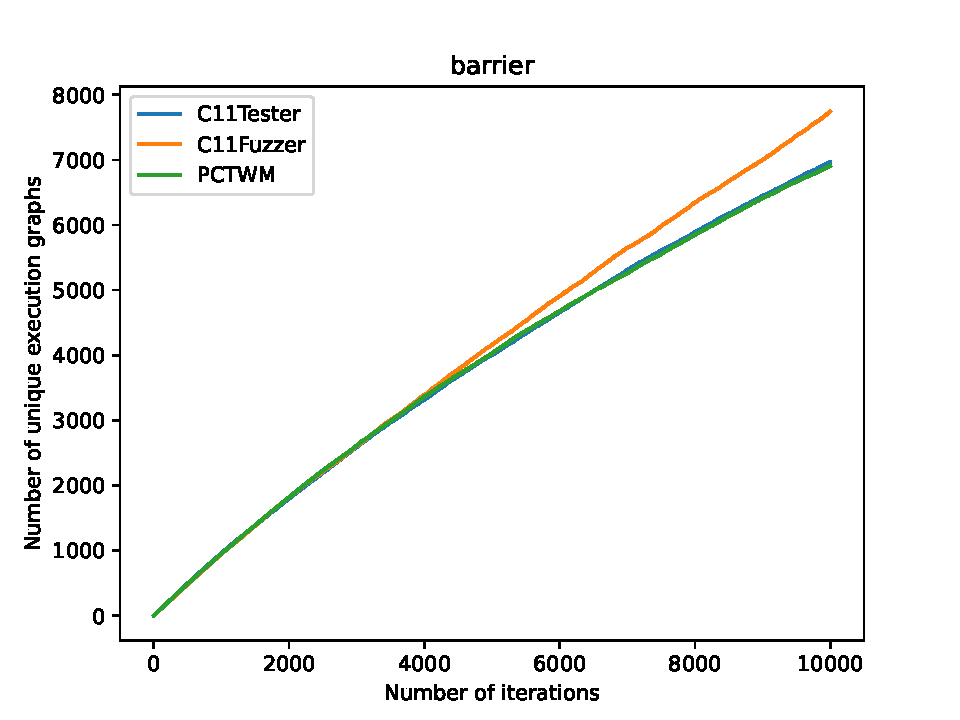
\includegraphics[width=\textwidth]{figure/pctwm/barrier.pdf}
		\caption{barrier}
		\label{pctwm-barrier}
	\end{minipage}
	\hfill
	\begin{minipage}{0.45\textwidth}
		\centering
		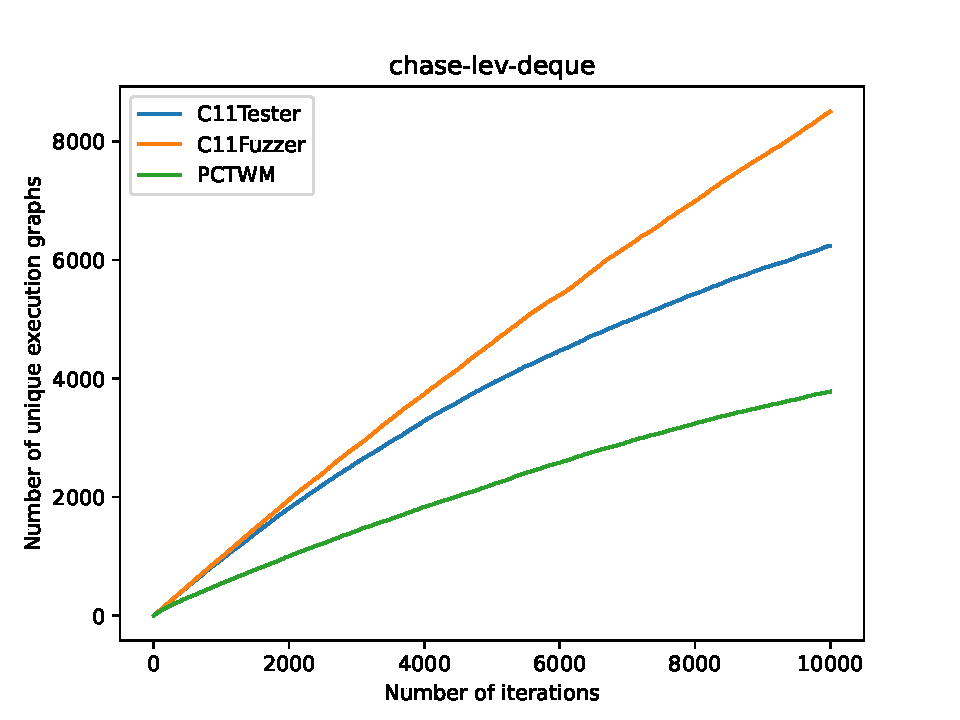
\includegraphics[width=\textwidth]{figure/pctwm/chase-lev-deque.pdf}
		\caption{chase-lev-deque}
		\label{pctwm-chase-lev-deque}
	\end{minipage}
	\vspace{0.5cm}

    \begin{minipage}{0.45\textwidth}
		\centering
		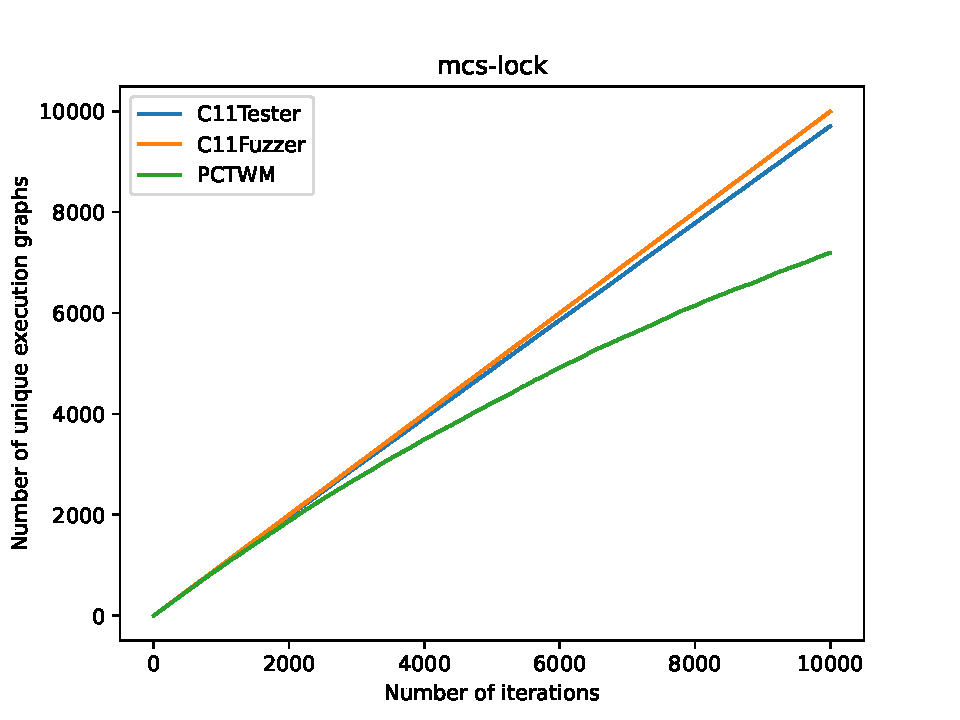
\includegraphics[width=\textwidth]{figure/pctwm/mcs-lock.pdf}
		\caption{mcs-lock}
		\label{pctwm-mcs-lock}
	\end{minipage}
	\hfill
	\begin{minipage}{0.45\textwidth}
		\centering
		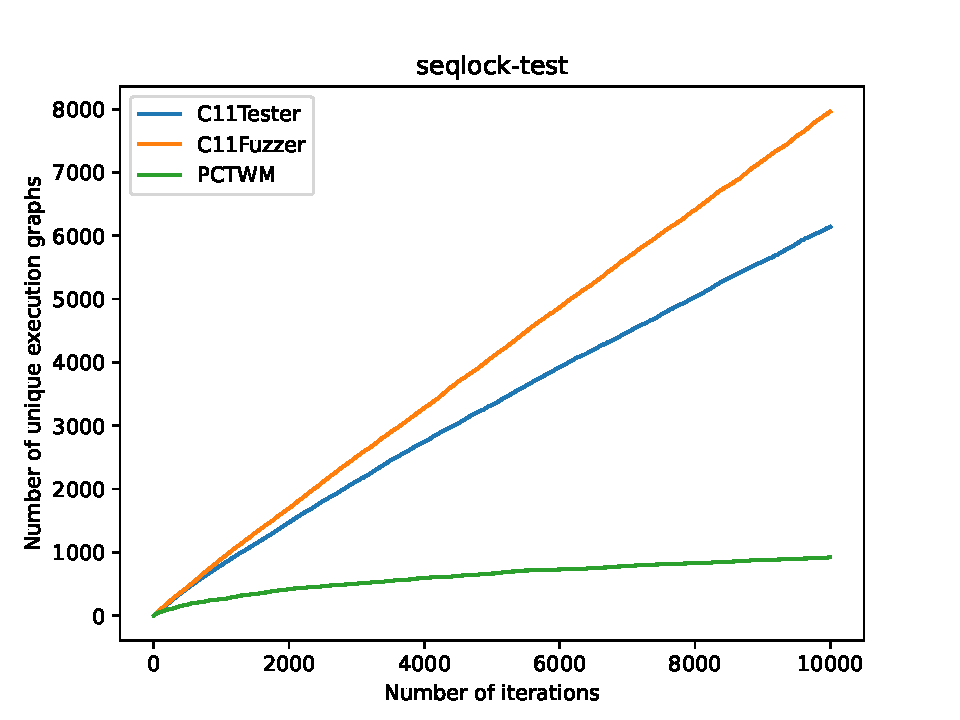
\includegraphics[width=\textwidth]{figure/pctwm/seqlock-test.pdf}
		\caption{seqlock-test}
		\label{pctwm-seqlock-test}
	\end{minipage}
	\vspace{0.5cm}

    \begin{minipage}{0.45\textwidth}
		\centering
		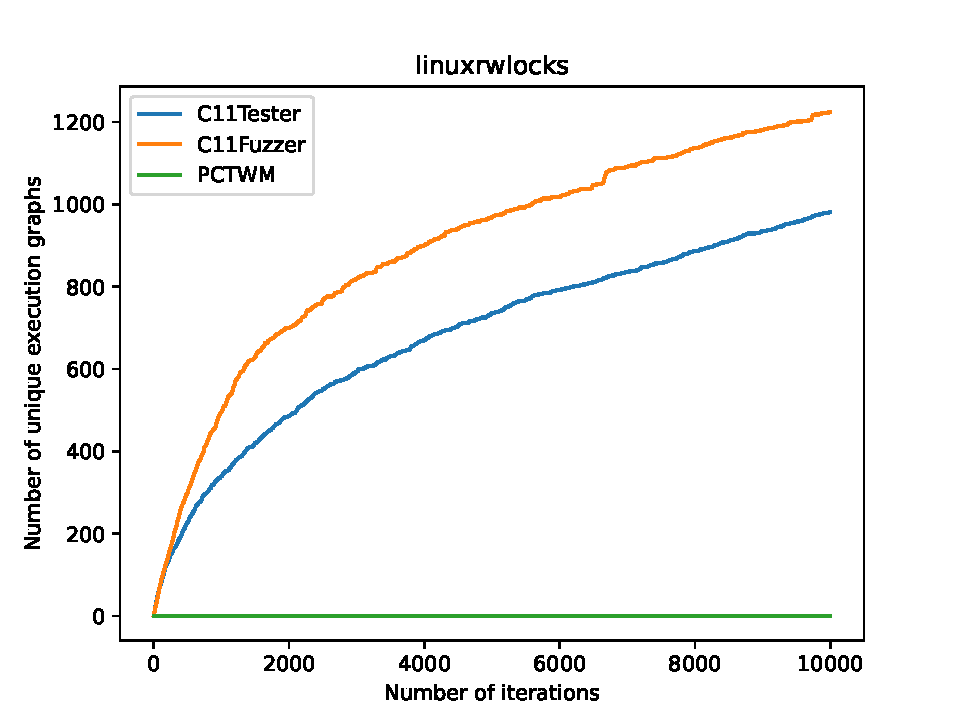
\includegraphics[width=\textwidth]{figure/pctwm/linuxrwlocks.pdf}
		\caption{linuxrwlocks}
		\label{pctwm-linuxrwlocks}
	\end{minipage}
	\hfill
	\begin{minipage}{0.45\textwidth}
		\centering
		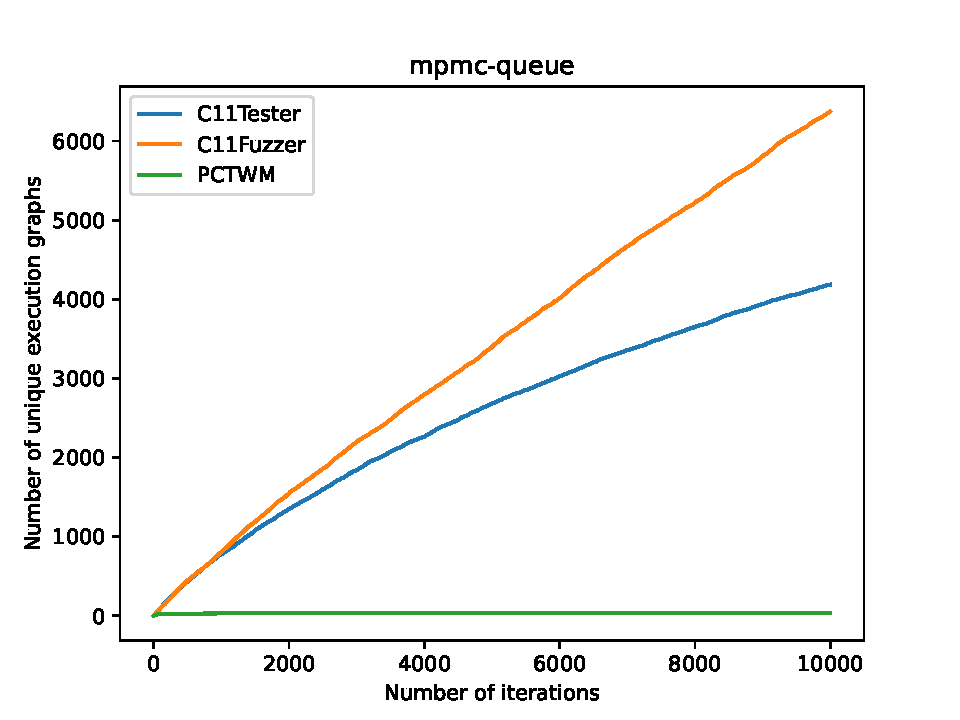
\includegraphics[width=\textwidth]{figure/pctwm/mpmc-queue.pdf}
		\caption{mpmc-queue}
		\label{pctwm-mpmc-queue}
	\end{minipage}
	\vspace{0.5cm}

\end{figure}


\subsection{\ref*{RQ:bug}: Bug hitting rate}
\subsection{\ref*{RQ:overhead}: Real-world applications}



\burcu{TODO: Discuss the results/plots. What do we observe? What can we say about the results?}

